\section{Decentralized Virtual Worlds Management}
\label{sec:decentr-virt-worlds}
Our response to the demand for an efficient metaverse platform capable
of 3D interactions among entities is the new version of \sol.  Its key
characteristic is the ability to distribute the cost associated with
the management of its metaverse among the hosts participating in
it. This is made possible through the decentralization of heavy
processes like collision detection, computation of physics, as well as
communication among the large number of nodes that participate in the
metaverse. In the following, we present the main characteristics of
the architecture and of the protocol enabling such
decentralization. 

\subsection{Definitions}
\label{sec:definitions}
The \sol metaverse consists of a set of \emph{entities}, each
belonging to one of three categories: \emph{avatars}, \emph{objects},
and \emph{sites}. Avatars are the main actors of the metaverse as they
are the only entities that are capable of autonomous movement. In most
cases they are virtual representations of the users of the metaverse
and are directly controlled by them using the navigator platform
described in Section~\ref{sec:navigator}.  Objects, on the other hand,
are virtual representation of entities from the real world such as
furniture, books and whatever object may be moved or picked up by an
avatar. Avatar and objects may also be robotic-like entities 
controlled by user-defined software components. Finally, sites
constitute the basic building blocks of the metaverse and represents
portions of the virtual space that may be occupied by objects or in
which avatars can roam.

Avatars, objects, and sites are all associated with 3D-descriptions,
each consisting of a mesh- or prims-based model, a set of textures,
and, in the case of avatars or objects, also of an animation.  Such
3D-descriptions constitute the basis for the rendering of entities in
the navigator platform.

The state of an entity in the metaverse is determined by an
\emph{entity descriptor}, from now on referred to simply as
\emph{descriptor}. An entity's descriptor can contain information
regarding its position, its physical properties, and whatever is
needed to display the entity and compute its interaction with the rest
of the metaverse. For example, a descriptor containing a key frame can
be used to synchronize animations, videos, and so on. Moreover,
filtering descriptors defining areas (concentric spheres, hierarchical
partitioning, cells) associated with a level of detail or a set of
visible objects may be used to achieve efficient on-demand streaming
while satisfying view-dependency criteria. Finally, descriptors may
contain load-balancing information regarding, for example, the
available resources or serving capabilities of a
host~\cite{cavagna}.
% auto-regulate the network load
Table~\ref{tab:desc} shows a sample descriptor containing the
most relevant information. Although the descriptor is shown as a
single object, the \sol implementation may split it into several
descriptors regarding, for example, physical properties,
location, or level of details in order to reduce communication cost.


% Each entity is associated with a unique identifier,
% with a set of properties such as its size or its location in the
% virtual world and with 

% In the following, we furth

%  Each object is
% associated with a unique identifier (UID) and may be classified into
% groups: \emph{roaming} or \emph{static}. Roaming objects may roam
% around the virtual world, and interact with it. Static objects on the
% other hand are associated with a fixed position in the virtual
% space. In this version of the specification, we consider only one type
% of roaming and one type of static objects, respectively,
% \emph{avatars} and \emph{sites}.

% Objects may be described with several levels of details. In this
% version of the specification, we concentrate on a very coarse-grained
% subdivision between two such levels: a complete description,
% comprising a full-fledged 3D model, and a simple predefined shape with
% no textures that is encoded in an \emph{object descriptor}

% % Nonetheless, the protocol can
% % easily support several levels of details with only minor
% % modifications. The two levels we consider consist of a \emph{complete
% %   description} of the object and of a an% \df{This will change. Ultimately we are going to have:
% %   descriptor, and 3dData, which in turn consists of mesh, texture, and
% %   animation.}.

% The object descriptor, on the other hand, consist of the minimal
% information required to display a rough representation of the object
% and includes the object's location, its shape, its size, its
% orientation, and its visibility radius, vRadius. The shape of the object is
% represented by an identifier that selects one from a set of predefined
% shapes; while its visibility radius identifies the distance from which
% the object should be visible in the absence of obstacles and without
% any visual aids. 


% The object descriptor of an object also keeps track of which hosts
% have recorded a copy of the object's 3D description. Specifically,
% each descriptor contains two fields associated with each of the files
% that constitute the object's 3D model. The first field is the latest
% known version number of the file, while the second is a list of hosts
% that are known to have cached a copy of the version of the file
% indicated in the first field.

% The object descriptor is the means through which the \sol protocol
% tracks the evolution of an object. To maintain consistency, each node
% descriptor should be modified by only a single object at a time.  For
% this reason, each descriptor also contains a sequence number that is
% incremented each time the descriptor is modified.  The general rule
% for modifying object descriptors in the \sol protocol is that each
% descriptor may be modified only by the site node that is responsible
% for the current location of the corresponding object. This is
% straightforward in the case of static objects (sites), but is somewhat
% more complex in the case of roaming objects (avatars), as these may
% roam move from one location to another and thus from one site node to
% another. 

% Specifically, in the case of roaming object, the node responsible for
% the object's location may not be the same as the node that is
% currently owning the object. Yet, the owner of the object should still
% be entitled to modify attributes of the object descriptor such as the
% shape or the files associated with the 3D model. Details about how
% this is achieved are given in Section~\ref{}. %  o make this
% % possible, we also define for roaming objects, an additional
% % \emph{static descriptor}\df{need a better name}, which includes all
% % the fields in the object descriptors excluding location and
% % orientation. The static descriptor of a roaming object can only be
% % modified by the owner of the object, while the object descriptor is
% % managed by the node responsible for the object location, as described
% % in Section~\ref{}. 

% Finally, in future versions of the protocol, the object descriptor may
% contain information required to implement progressive levels of
% details in the 3D representations of objects.  A summary of the fields
% included in an object descriptor is shown in Table~\ref{tab:desc}.

\begin{table}
\centering
\scriptsize
\begin{tabular}{|l|p{6cm}|}
\hline
  $\mathsf{UID}$ & universal identifier of the entity\\
  $\mathsf{seqNum}$ & sequence number\\
\hline
  $\mathsf{owner}$ & identifier of the node managing the entity\\
  $\mathsf{type}$ & site, avatar or object\\
  $\mathsf{loc}$ & location in the 3D space\\
  $\mathsf{ori}$ & orientation in the 3D space\\
  $\mathsf{shape}$& shape from a predefined set\\
  $\mathsf{box}$ & bounding box of the object\\
  $R_p$ & perceptibility radius: distance from which the object is
  visible in the absence of obstacles\\
  $R_b$ & radius of  smallest sphere enclosing the entity\\
  $\mathsf{objs}_a$ & list of entities attached to the current one\\
  \hline
  $f_1$ & first file of 3d-description \\
  $v_1$ & version number for first file\\
  $c_1$ & list of hosts that have cached $v_1$ of $f_1$\\
  ...& ...\\
  $f_n$& n-th file of 3d-description\\
  $v_n$& version number for n-th file\\
  $c_n$& list of hosts that have cached $v_n$ of $f_n$\\
  \hline
  ... & additional fields for progressive levels of details\\
  \hline
\end{tabular}
\fcaption{Example of a simple descriptor}
\label{tab:desc}
\end{table}

\subsection{Solipsis Hosts and Nodes}
From a practical viewpoint, the \sol platform is distributed over a
set of hosts that maintain information about every entity that is
currently present in the metaverse.  Each host is associated with a
single instance of the \sol platform, and throughout its lifetime, it
may create new entities or destroy previously created ones according
to the requests of the navigator component. Also, similar to an
entity, each host is associated with a unique identifier (UID).

Because each host may be responsible for several entities at the same
time, we define a \emph{(Solipsis) node} as the set of resources
dedicated to the management of a given entity. Each node encapsulates
information about the corresponding entity's descriptors as well as
the threads of control responsible for managing all the interactions
of the node with the rest of the \sol metaverse as well as with the
navigator platform.

\subsection{P2P Architecture}
\label{sec:p2p-architecture}
A fundamental aspect of \sol is its completely decentralized
architecture designed to accommodate large numbers of entities,
accessed by large numbers of users distributed over the Internet.  The
core of this decentralized architecture is a \ptp overlay network,
which is essentially a graph where nodes are connected by virtual
logical links, each of which may consist of several physical links in
the underlying IP network. These logical links may be laid out
according to some proximity metric so as to enable efficient storage
and retrieval of information.



Recent years have seen the emergence of a large number of \ptp overlay
networks, with different structures and capabilities.  In the context
of \sol, we leverage the potentialities of \ptp overlays by building
our metaverse on top of RayNet~\cite{beaumont}. Raynet is a
multi-dimensional overlay network based on the concept of Voronoi
tessellation. As shown in Figure~\ref{Fig:Overview}, each node in the
overlay is associated with a position in a multi-dimensional
space. Neighborhood relationships between peers are then determined by
the distance between the corresponding points in this
space. Specifically, two Raynet nodes are neighbors in the overlay if
the two corresponding points are neighbors in the Delaunay graph
comprising all the points associated with Raynet nodes.

\begin{figure}
\center
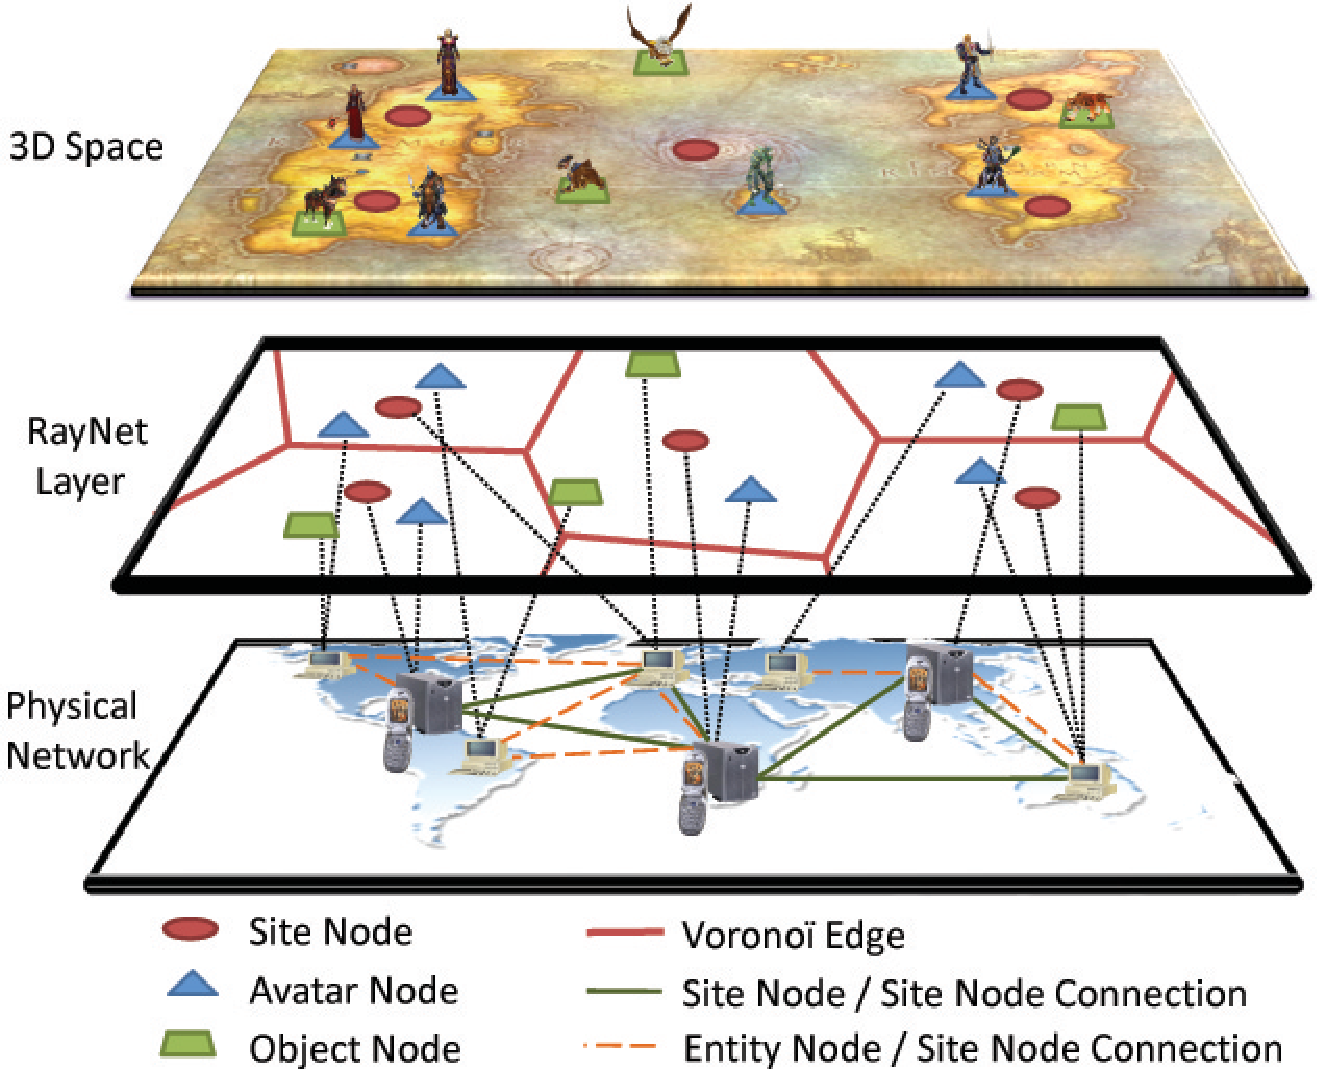
\includegraphics[width=3in]{Figures/Overview.pdf}
\fcaption{The p2p architecture showing the mapping of the Raynet layer
  on the virtual world layer according to the proximity of nodes in
  the virtual space. The host layer shows clients connected into a
  peer to peer scheme. Note that while the positions of avatars and
  objects are also shown, for clarity, on the Raynet layer, only site nodes
  actively join the RayNet and form the corresponding Voronoi diagram.}
\label{Fig:Overview}
\end{figure}

Given a set of generator points$\{p \in \Re^d\}$, the Delaunay graph
is obtained as the adjacency graph of the corresponding Voronoi
diagram, which in turn is a tessellation of the d-dimensional space
$\Re^d$. Specifically, the cell in the tessellation associated with a
point $p_x$ is such that it contains all the points that are closer to
$p_x$ than to any other generator point in the set. This property
enables Raynet to route to any node in the overlay by means of a
simple greedy approach. Moreover, the addition of
Kleinberg-like~\cite{ jk:smallworld} long-range links allows this
routing process to converge to its destination node in a
polylogarithmic number of hops on average.

Within the context of \sol, we use the Raynet structure to organize
\emph{site nodes} into a 3-dimensional overlay in which the positions
of nodes mimic those of the corresponding sites in the
metaverse.\footnote{Extensions of the metaverse architecture to higher
  dimensions are naturally supported by the Raynet overlay.} This
allows our architecture to exploit very simple protocols to manage the
interaction between avatars, objects and the sites they are currently
located in as we describe in the following.

\subsection{Decentralized physics computation}
\label{sec:decentr-phys-comp}
The choice of a \ptp overlay such as Raynet is motivated by our goal
to scale to metaverses containing very large numbers of entities,
possibly gathered within the same site or within an otherwise
small region of space. Organizing sites nodes into such an overlay,
however, is only half of the picture. \sol also incorporates a fully
decentralized protocol that distributes the cost associated with heavy
computations such as those regarding collision detection, physics, or
animation.


Each avatar node is responsible for computing its own position based
on physical criteria like its mass, momentum, and forces applied
by the entities in its surroundings. Our decentralized approach allows
it to achieve this result by taking into account only a small set of
3D models: those associated with the current site and with the
entities that are in the avatar's immediate surroundings. 
For example, in the case of collisions, each avatar may immediately
rule out the entities that are at a distance that is greater than the
radii, $R_b$, of the spheres enclosing its and their own bounding boxes
plus a configurable safety distance.

% the one
% associated with the current site and those of

% \jr{\bf{detecting its collision with 3D models of the scene and for
%     computing its position in the space }}computing its position of its avatar in the
% multiverse, based on its physical properties and those of the entities
% around it.

The basis for this decentralized computation of physics is a
communication protocol that allows nodes to exchange information about
entities' positions with three levels of heartbeat messages. Critical
information that is required for the computation of collision
detection is exchanged directly in a peer-to-peer fashion between the
avatars that may potentially collide with each other, based on the
size of their bounding boxes. Less critical information that is
nonetheless necessary to provide the navigator with a clear snapshot
of the current scene state is instead propagated indirectly, in a
multi-hop fashion. Finally, information about distant objects or
objects that have just joined the metaverse is propagated by site
nodes to the avatars within their cells at a significantly lower
frequency.

An avatar joining \sol contacts the site node responsible for its
joining - or latest - location. Although the avatar is not part of the
overlay, it can easily do this by using the Raynet to route a message
containing its descriptor to the site node that is closest to its own
position. This node then reacts by providing the avatar with the
descriptors of the entities that are potentially visible from its
location. From this point on, the avatar and site nodes exchange this
information periodically to implement the low frequency updates
described above.  An analogous mechanism is used to manage the
positions of object nodes. The use of the Raynet always allows avatars
and objects to contact the right node as they move from site to site.

In addition, avatar and object nodes interact with the avatars and
objects around them in order to exchange the critical up-to-date
information about the entities that may collide with them.  Also,
while sending an update to a nearby node, avatar and object nodes also
include information received from other nearby nodes that are not
within collision distance of the destination node; thus implementing
the second level of \ptp updates. % Finally, we observe that an avatar
% or object node may compute the set of entities within collision
% distance by comparing the their distance with the size of its and the
% neighboring entities' bounding boxes the avatar or object and the size
% of the relative bounding boxes as specified in the corresponding
% descriptors.



 
\subsection{Dynamic Object Management }
\label{sec:manag-inan-objects}
While avatars are the main actors in the \sol environment, objects
also play an important part as they can interact with avatars, be
picked up, be moved from one location to another, or even move freely
through space subject to gravity or other forces, or according to a
script of animation. This requires our protocol to determine the
current position of objects in addition to that of avatars. This is
achieved through a combination of three mechanisms that depend on the
state the object is currently in.

Let us consider an object that is currently stationary within a site
$S$'s cell. The position of the object is maintained by $S$'s site
node, which also maintains the main copy of the object's
descriptor. As soon as an avatar tries to interact with the object, by
moving it or picking it up, its avatar node sends a request to the
site node to take over responsibility for the object. The site node
grants such responsibility to the first avatar requesting it,
according to the order in which requests reach the site node.

When permission to take over the object is granted, the object is
dynamically detached from the site and attached to the avatar. The
corresponding descriptors are updated, and the avatar nodes starts
computing physics and maintaining the descriptor for the object. Note
that physics computation need not be performed by site nodes, in that
an object can only be attached to a site when it is in static
equilibrium.

After interacting with the object, the avatar may pass the object on
to another avatar, or leave it in the current or in a different
site. In the former case, the recipient of the object takes over its
management, and starts computing its physics, and animation, and
updating its descriptor.  In the latter, on the other hand, the object
may be left in a stationary or in a dynamic state. If the object is
stationary, then the site may take control of its descriptor and
manage it without computing any physics. If, on the other hand, the
object is moving, or subject to forces that are not in equilibrium,
then a new object node with a corresponding thread is instantiated on
the host associated with the avatar to which the object was
attached. This new object node takes responsibility for managing the
object's movements and updating its descriptor until it is picked up
by a new avatar or until it reaches an equilibrium state at some site.
It should be noted that a host may keep managing an object, even if
the associated avatar is at a distant location. This allows hosts to
manage robotic-like entities that are controlled by user-defined
software components, e.g. by associating streaming video to
objects.

\subsection{Decentralized 3D-Model Sharing}
\label{sec:decentr-3d-models}
The architecture we have described so far assumes that nodes are able
to retrieve the 3D-description of entities in order to compute
collisions and display the entities after filtering them based on the
information in their descriptors. In the following, we describe our
mechanism for maintaining and retrieving these 3D-descriptions. As
with the rest of the protocol, our goal is to distribute the cost of
managing 3D-descriptions among \sol participants.

%  An important task
% performed by the threads of control associated with \sol nodes is the
% management of the 3D-descriptions associated with entities. This
% involves both modifying the current entity's description, for example
% by adding a new animation, and, in the case of avatar nodes,
% downloading other entities' descriptions so that they can be displayed
% by the navigator component.


3D-descriptions are managed by the nodes responsible for the
corresponding entities, and may be downloaded by any node that needs
to display the object or perform collision detection. However, having
all hosts download a given 3D-description from the node responsible
for its entity would place an unnecessary load on the corresponding
host. We address this issue, by having \sol nodes cache previously
downloaded descriptions. This allows them to offer them for download
to other \sol nodes running on the same or remote hosts.

All the nodes residing on a host, store their own 3D-descriptions as
well as those of other visible objects in a shared repository
(depicted in Figure~\ref{Fig:host}) that is accessible by all the nodes
running on the same host. Moreover, each node records in its
entity's descriptor a list of the hosts that currently hold a copy of
any of the files that constitute the associated 3D description.
Whenever a node caches a 3D-description, it informs the node
responsible for the entity, which then updates the corresponding
descriptor to include a reference to the new copy and then propagates
it with its subsequent heartbeat messages. Similarly, when a
node detects that a host listed in the descriptor does not have the
current copy of an entity's description, it sends a message to the
corresponding node, which updates the descriptor accordingly.

\subsection{Managing Disconnections}
The architecture of \sol is designed to tolerate unexpected
disconnections of hosts throughout its operation. First, site nodes
always cache the 3D-descriptions, in addition to the descriptors, of
neighboring site nodes. This allows the RayNet to manage the
disconnection of a site node by automatically assigning its management
to any of the neighboring site nodes. The disconnection of an avatar
or object node, on the other hand, is treated by attaching the object
or avatar to its current site and by leaving it in a stationary state
until the corresponding user reconnects.









%%% Local Variables: 
%%% mode: latex
%%% TeX-master: MMVE
%%% End: 
